%
% ---------------------------------------------------
%
% Proyecto Final de Carrera: EMIR
% Autor: Pedro Hernández Martín <alu3679@etsii.ull.es>
% Capítulo: Estado del arte
% Fichero: Cap2_estado_del_arte.tex
%
% ----------------------------------------------------
%

\chapter{Motivación} \label{chap:motivacion}
EMIR, que actualmente está entrando en su etapa de fabricación y en fase de AIV, será uno
de los primeros instrumentos para usuarios en común para el GTC, el telescopio
de 10 metros del proyecto GRANTECAN ubicado en el Observatorio del
Roque de los Muchachos (Islas Canarias, España). EMIR está siendo construído por
un Consorcio de institutos españoles y franceses liderado por el IAC. 
EMIR está diseñado para llevar a cabo una de las
metas centrales de los telescopios de 10 metros, permitiendo a los
observadores obtener espectros para un gran número de fuentes tenues de una
forma temporalmente eficiente. EMIR está diseñado para operar principalmente
como un MOS en la banda K, pero ofrece un amplio rango de modos de observación,
incluyendo imágenes y espectroscopía, ambos de larga fisura y multiobjeto, en
una longitud de onda en un rango de 0.9 a 2.5 micrómetros. Está equipado con dos
subsistemas innovadores: una máscara robótica reconfigurable multi-ranura y
elementos dispersivos formados por la combinación de prismas convencionales y
rejillas difractantes de alta calidad, ambos localizados en el corazón del
instrumento. 
%El presente estado de desarrollo, el rendimiento esperado, y la
%planificación para la explotación científica están descritos y discutidos. 
El desarrollo y la fabricación de EMIR está financiado por el GRANTECAN y el Plan
Nacional de Astronomía y Astrofísica.

La nueva generación de telescopios ópticos de 10 metros cercanos al infrarrojo,
%actualmente bajo construcción, 
con la intención de sondear el Universo más
profundamente, mantienen la promesa de proveer, por vez primera, una visión
directa de los procesos que dieron forma a la creación de estrellas, galaxias, y
el propio Universo. Proveerán también, por vez primera, la capacidad de detectar
y aislar estrellas extragalácticas y regiones de formación de estrellas con una
sensibilidad sin procedentes y poder de resolución, ambos espaciales y
espectrales. Un esfuerzo colectivo de instrumentación está en camino para
permitir a estas nuevas infraestructuras su uso a pleno potencial. Las
capacidades científicas de los nuevos telescopios se estiman como enormes, no
sólo por su gran área de recolección de fotones, sino especialmente por los
nuevos instrumentos, los cuales, debido a importantes avances tecnológicos, se
espera que sean órdenes de magnitud más eficientes que sus homólogos de hoy en
día. Como añadidura, estos retos tecnológicos establecerán los primeros pasos
hacia la construcción de instrumental para la próxima generación de telescopios
de más de 30 metros, que se encuentran en la fase principal de su diseño
conceptual.

El Observatorio del Roque de los Muchachos, en la isla de La Palma, operado por
el IAC, es el lugar de emplazamiento del
Gran Telescopio Canarias (GTC) de 10 metros, que vio su primera luz en 2007. El
GTC será el mayor telescopio óptico del mundo. Junto con este esfuerzo, una
asociación de instituciones españolas y francesas dedicadas a la investigación
está trabajando en el diseño y construcción de EMIR, un avanzado
espectrógrafo-multiobjeto NIR para el GTC, objeto central de interés de este PFC.

EMIR (Espectrógrafo Multi-Objeto Infrarrojo) es un espectrógrafo de campo ancho
de usuario común operando en las longitudes de onda cercanas al infrarrojo (NIR)
0.9-2.5 micrómetros, usando máscaras multi-ranura criogénicas como selectores de
campo. Las especificaciones están listadas en la Tabla \ref{tabla:especificaciones}. 
EMIR proveerá al GTC de imágenes de rendija larga y espectroscopías de varios
objetos. El consorcio EMIR está formado por el IAC, la Universidad Complutense
de Madrid (UCM, España), el Laboratorio de Astrofísica de Marsella-Provenza
(OAMP, Francia) y el Laboratorio de Astrofísica de los Pirineos Medios (LAOMP,
Francia). 

\begin{table*}
\centering
\begin{tabular}{|l l|}
\hline
Wavelength range & 0.9-2.5 $\mu$m \\
Optimization & 1.0-2.5 $\mu$m \\
Observing modes &  Multi-object spectroscopy \\
& Wide-field Imaging \\
Top priority mode &  K band Multi-object spectroscopy \\
Spectral resolution & 5000,4250,4000 (JHK) for 0.6$''$ (3-pixel) wide apertures \\
Spectral coverage & One observing window (Z, J, H or K) per single exposure \\
Array format & 2048$\times$2048 HgCdTe (Rockwell-Hawaii2) \\
Scale at detector &  0.2 arcsec / pixel \\
OH suppression & In software \\
Image quality  & $\theta_{80}< 0.3$ arcsec \\
\multicolumn{2}{|c|}{\textbf{Multi-object spectroscopic mode}} \\
Slit area & 6$\times$4 arcmin, with approx. 50 slitlets of $\sim$7'' long and width \\
          & varying between 0.4 and 1 arcsec \\
Sensitivity & K$<$20.1, t=2hrs, S/N=5 per FWHM (continuum) \\
            & F$>$1.4$\times$10$^{-18}$erg$^{-1}$s$^{-1}$cm$^{-1}\AA^{-1}$, t=4hr, S/N=5 per FWHM (line) \\
\multicolumn{2}{|c|}{\textbf{Image mode}} \\
FOV & 6$\times$6 arcmin \\
Sensitivity &  K$<$22.8, t=1hr, S/N=5, in 0.6$''$ aperture  \\
\hline
\end{tabular}
\caption{Especificaciones de alto nivel en EMIR}
\label{tabla:especificaciones}
\end{table*}

EMIR proveerá a la comunidad de usuarios de GTC con nuevas capacidades clave de
observación. Se espera que sea uno de los primeros espectrógrafos criogénicos
multiobjeto completos (MOS) en un telescopio de 10 metros, de manera que será
capaz de observar en la banda K a 2,2 micrómetros sin la desventaja del alto
fondo instrumental común en otros instrumentos conceptualmente similares.
Algunos MOS NIR similares existentes o planificados para otros telescopios, no
son enfriados y alcanzan hasta los 1,8 micrómetros solamente. Extender las
capacidades de un MOS hasta los 2,2 micrómetros es el siguiente paso natural en
el diseño de este instrumental. EMIR abrirá, por primera vez, el estudio de la
naturaleza de galaxias muy lejanas con tendencia al rojo más allá de z=2 con
una profundidad y campo de visión sin precedentes. Con estas tendencias al rojo,
el resto de galaxias bien estudiadas, en particular, la fuerte línea H alfa, se
mueve a la banda K, permitiendo diagnósticos clave sobre la historia de la
formación de estrellas en el Universo. EMIR permitirá puentear los estudios
extensivos de tendencias al rojo más bajas llevados a cabo en los años noventa
con telescopios de 4 metros y aquellos superiores a z=6 planeados para el futuro
próximo usando longitudes de onda pertenecientes al lejano infrarrojo
milimétricas. EMIR también proveerá un vínculo entre las capacidades
espectroscópicas actuales y aquellas que serán disponibles una vez que el
Telescopio Espacial James Webb (JWST) esté operativo a finales de ésta década.

El diseño de EMIR ha sido ampliamente determinado por los requerimientos de su
conductor científico principal, el estudio de galaxias tenues muy distantes, el
proyecto GOYA, anteriormente conocido como COSMOS. Aún siendo un instrumento de
usuario común, ha sido diseñado para ser conocido por la mayoría de la gran
comunidad astronómica. Es, por lo tanto, un instrumento versátil que cumplirá
con una amplia mayoría de proyectos científicos que comprenden desde los cuerpos
estelares extragalácticos, a la astronomía del Sistema Solar interestelar.

La construcción de EMIR impulsa los retos de la instrumentación para los grandes
telescopios hacia nuevos límites. La apertura de 10 metros del GTC se traduce en
una gran superficie física focal.  Emparejando las imágenes dadas por el
telescopio con el pequeño tamaño de los detectores de hoy en día, requiere
grandes ópticas con cámaras rápidas. Las grandes y pesadas ópticas necesitan un
diseño mecánico avanzado y un buen modelado para reducir la flexión a niveles
aceptables. Para trabajar en una región más allá de los 1,8 micrómetros, el
sistema óptico de EMIR y su estructura mecánica, serán enfriados a temperaturas
criogénicas. Un módulo clave de EMIR es una unidad de máscara criogénica que
permite varias configuraciones diferentes de máscaras multi-ranura, disponibles
cada noche, apropiado para las observaciones en cola intencionadas en el GTC,
sin tener que calentar el espectrógrafo. Todos los aspectos ya mencionados,
necesitan esfuerzo en desarrollo, debido a que la tecnología no está disponible
ó no se puede utilizar para soluciones ya existentes. 

\section{Problema a tratar}

El ``sistema robótico reconfigurable de rendijas'' con el que cuenta EMIR
presenta una estructura rectangular de 240 segundos de arco de ancho y 400
segundos de arco de alto. En el interior de este espacio se encuentran 55 pares
de barras horizontales, cuya altura es de $400/55$ ($\sim$7.27) segundos de arco.
En la Figura \ref{fig:CSUreal} se observa este sistema físicamente.
Cada pareja de barras se desplaza horizontalmente de forma independiente permitiendo
dejar un espacio entre ellas y observar el objeto espacial que se desee, o
bien cerrarse del todo para no medir nada en ese punto; de esta forma es posible
configurar cada par de barras para medir hasta 55 elementos simultáneamente (ver
Figura \ref{fig:CSU0}). 
A este subsistema de barras se le conoce como CSU (Configurable Slit Unit).

\begin{figure}[!htb]
\centering
\subfloat {
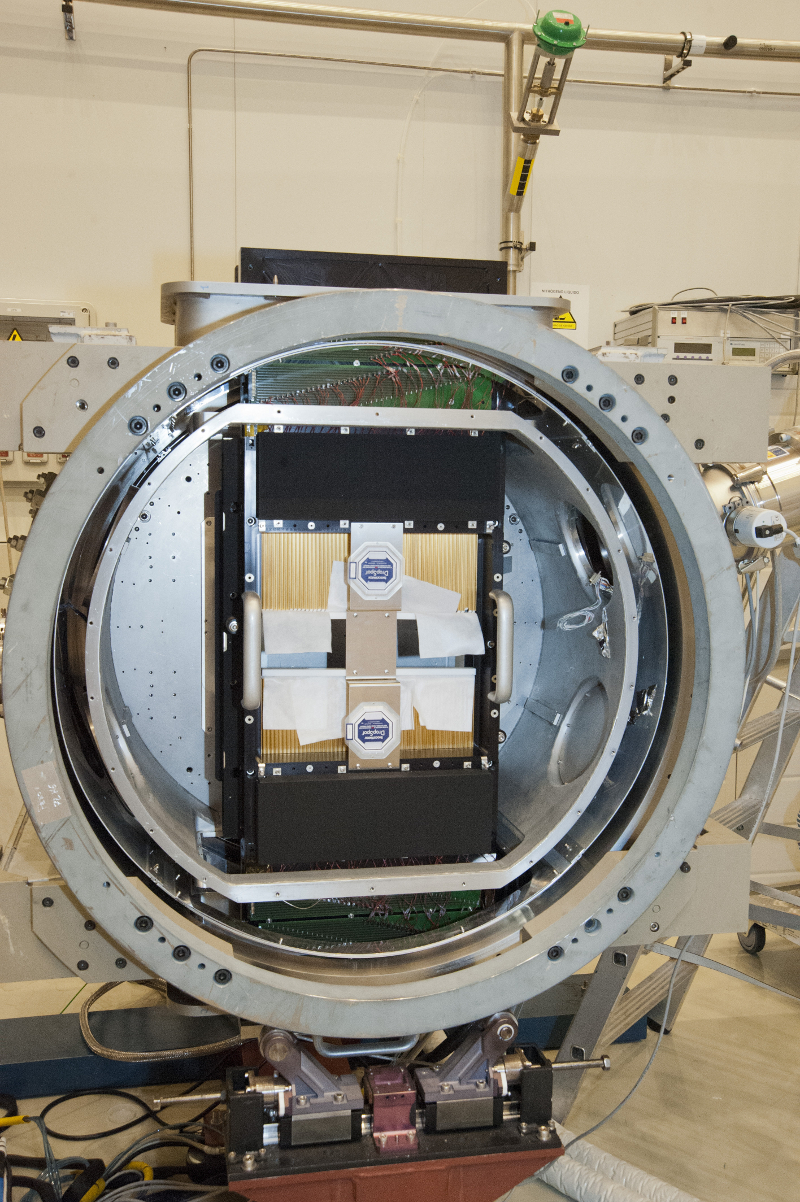
\includegraphics[height=0.5\linewidth]{DSC_9546}}
\subfloat {
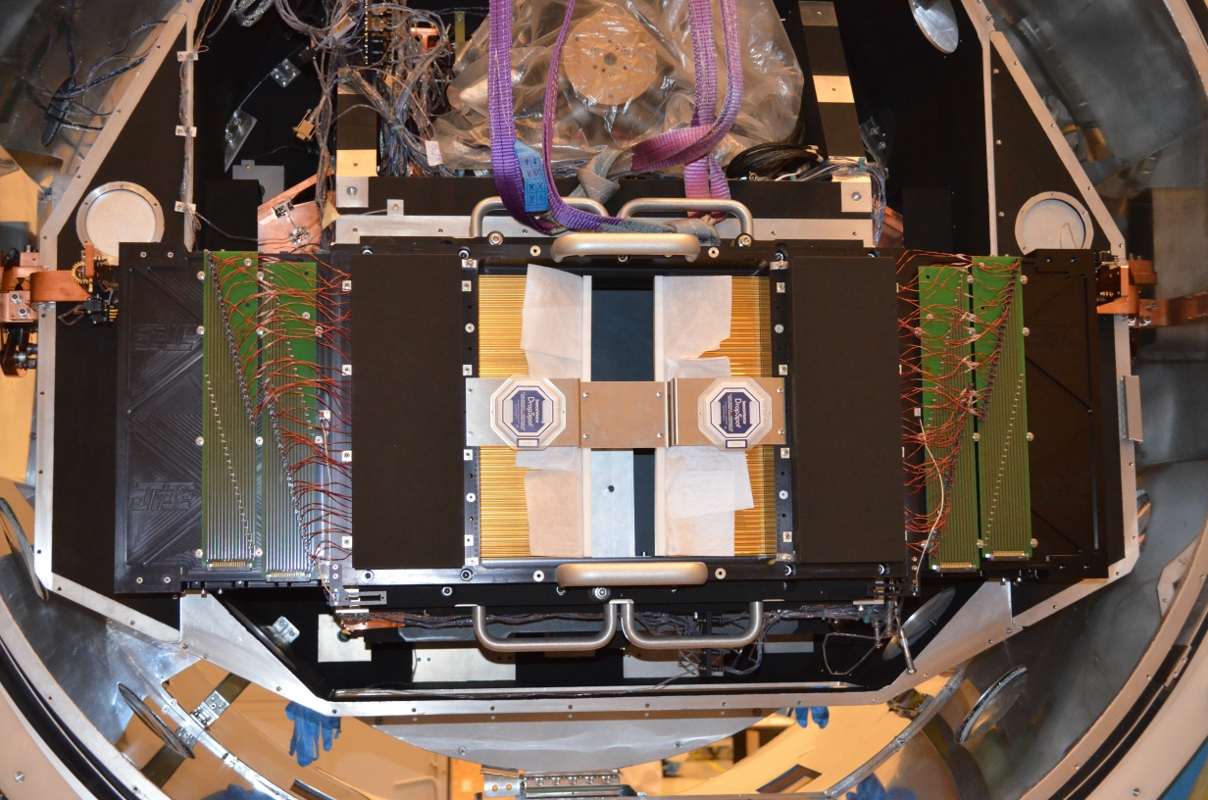
\includegraphics[width=0.7\linewidth]{DSC_0750}}
\caption{Unidad de rendijas configurables de EMIR}
\label{fig:CSUreal}
\end{figure}

EMIR rotará alrededor de su eje óptico durante el apuntado y operación, llevando
consigo a la CSU.  A efectos prácticos, esto significa que la CSU puede
configurarse en cada posición de apuntado del telescopio con ángulo de posición
en el rango [0,180] según las necesidades del usuario, como se muestra en la Figura
\ref{fig:CSU1}. Al ser simétrica, abarca todo el rango de giro posible, y puede 
estar colocada en cualquier punto del espacio visible (área de cielo observable
de dimensiones mucho mayores que las del subsistema). Llamamos ``apuntado'' a
una posición concreta de la CSU, especificada por un centro $(x,y)$ y un ángulo
de rotación, junto con la configuración de cada una de las 55 barras.

\begin{figure}[!htb]
\centering
\subfloat[CSU] {

\includegraphics[height=0.5\linewidth]{CSU}
\label{fig:CSU0}}
\subfloat[Rotación de la CSU] {
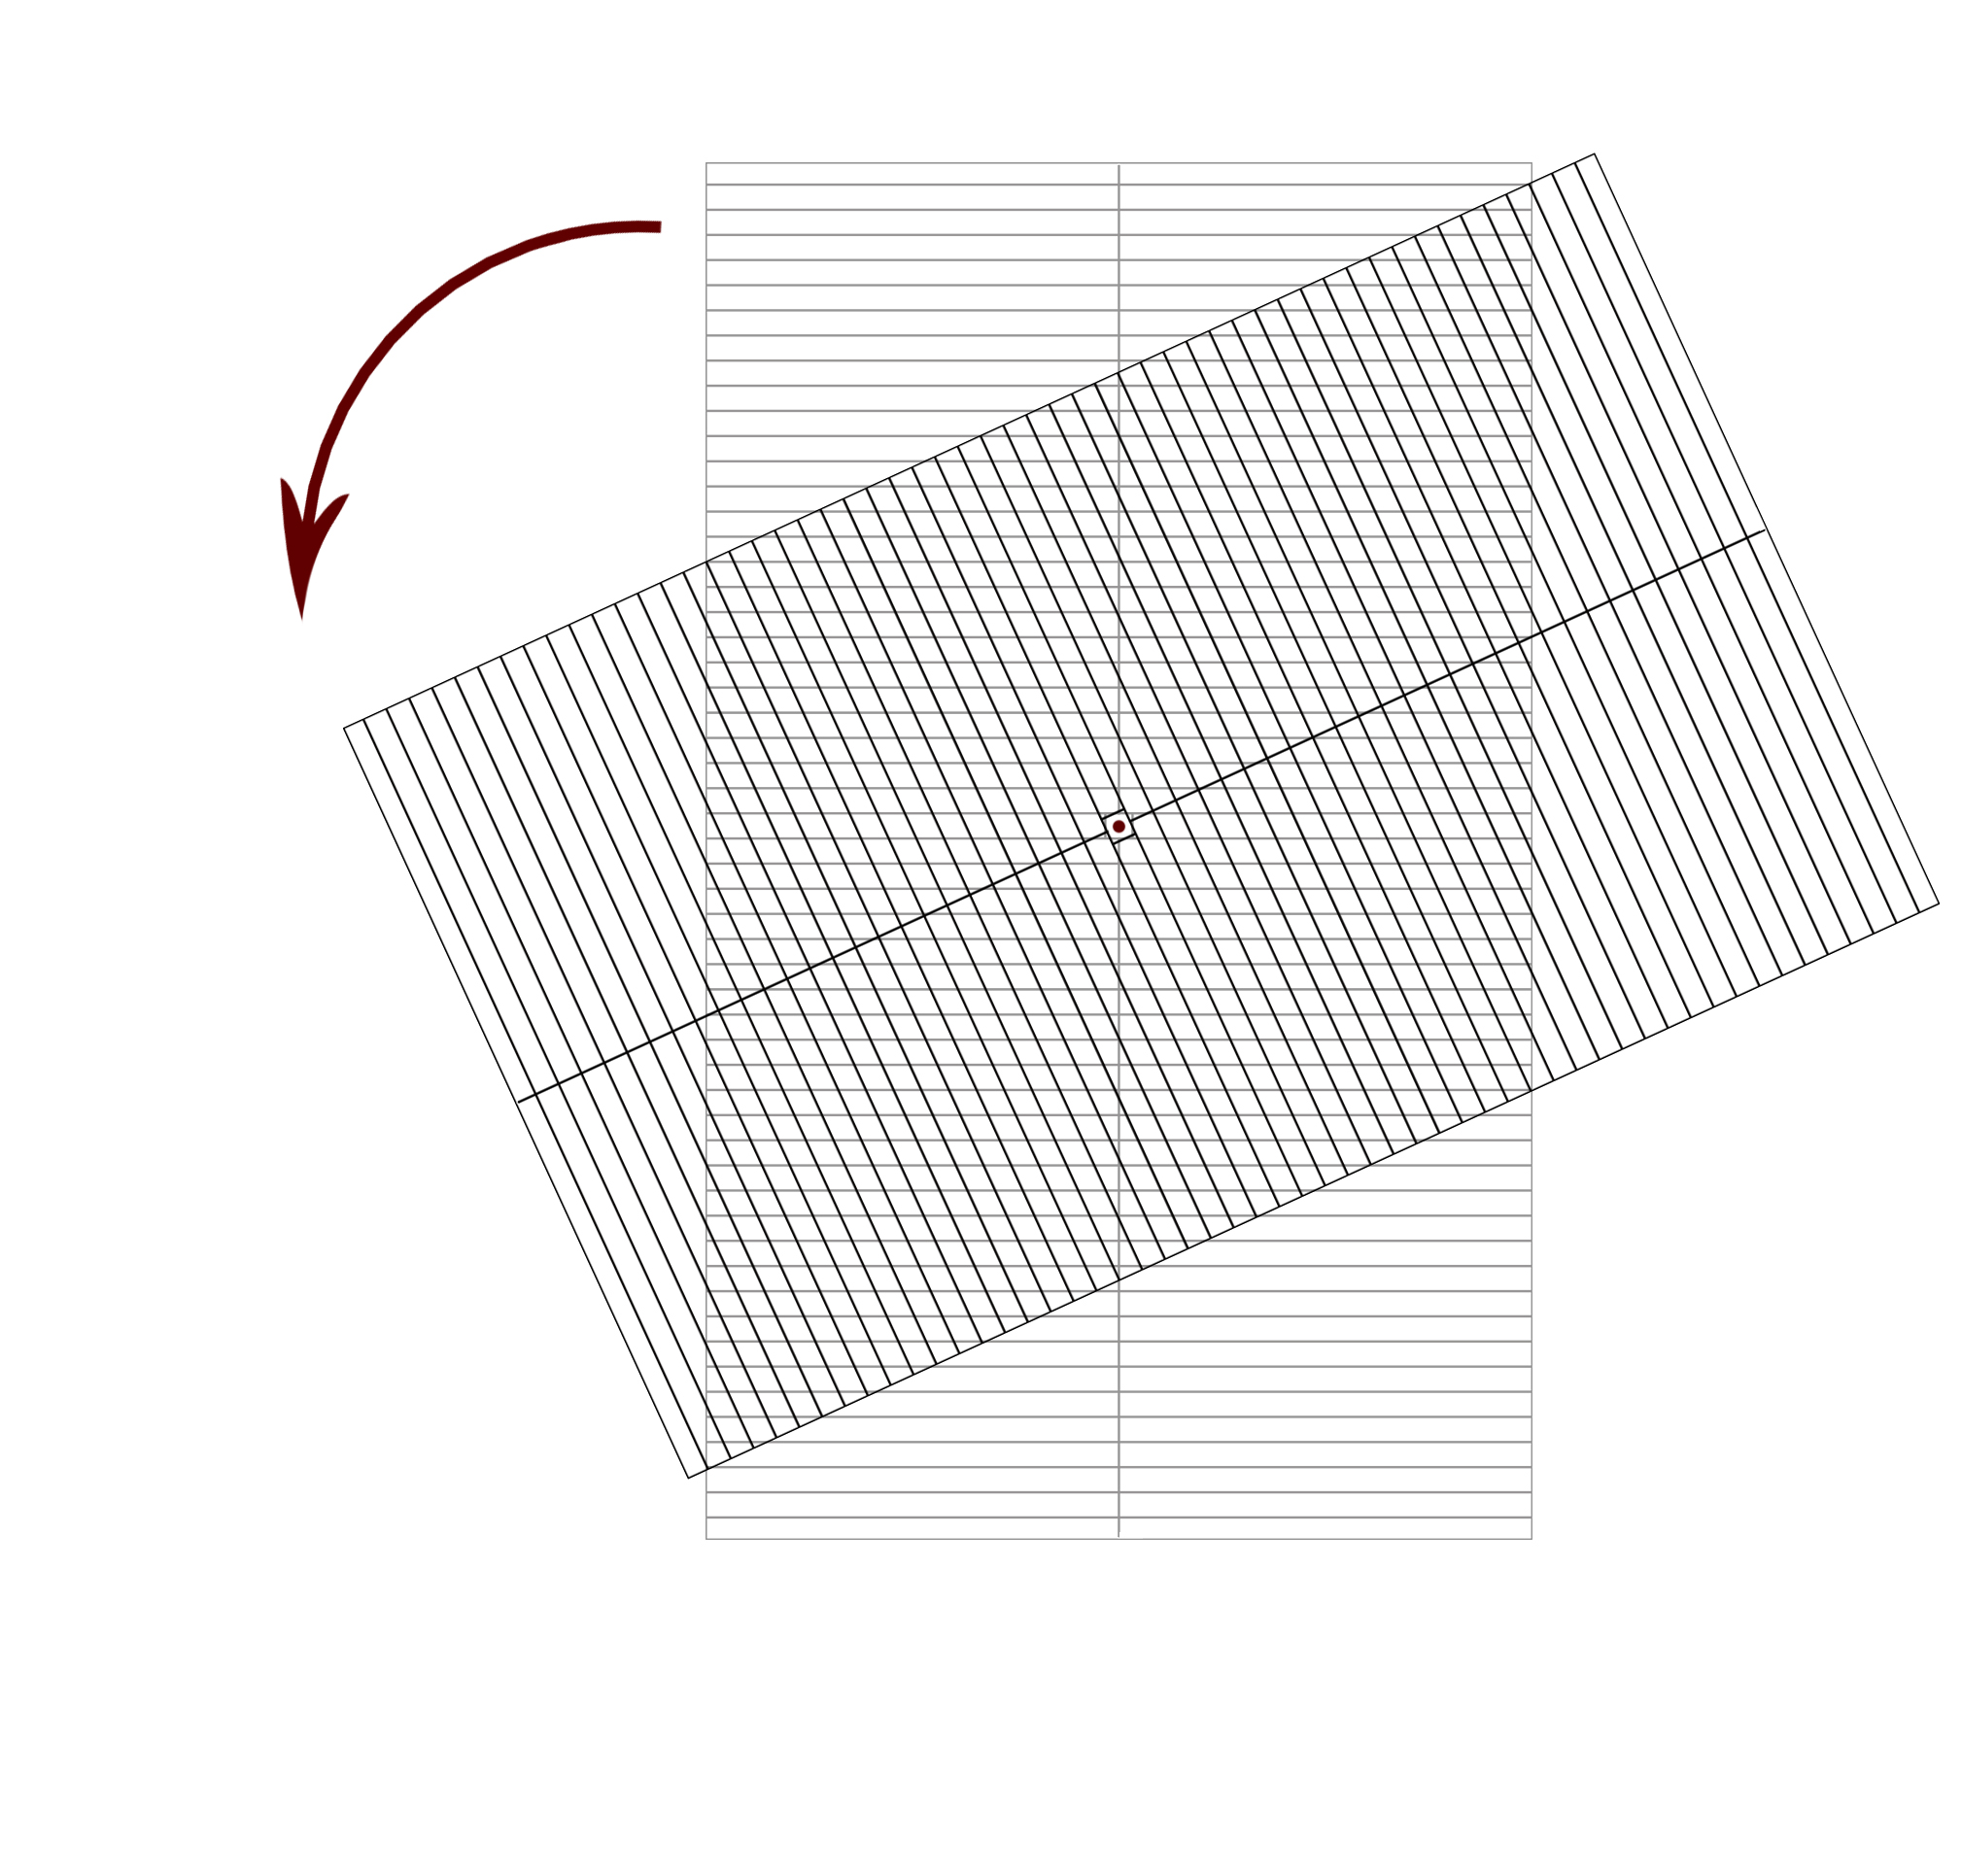
\includegraphics[width=0.5\linewidth]{CSU-giro}
\label{fig:CSU1}}
\caption{Representación gráfica de una CSU}
\end{figure}

Generalmente, para observar todos los objetos de interés astronómico de un
determinado campo es necesario utilizar más de un apuntado. Debido a que el
proceso de observación (medida) en cada apuntado de la CSU es muy lento, se hace
necesario minimizar el número de apuntados para cubrir todos, o al menos la
mayoría de  objetos de alta prioridad.  Para solucionar este problema se ha
desarrollado en el marco de este PFC una aplicación escrita en C++ que, dada una
entrada de puntos a medir, devuelve una lista de apuntados que resuelven el
problema. La Figura \ref{fig:CSU2} muestra un ejemplo de apuntado para cuatro
objetos.

\begin{figure}[!htb]
\centering
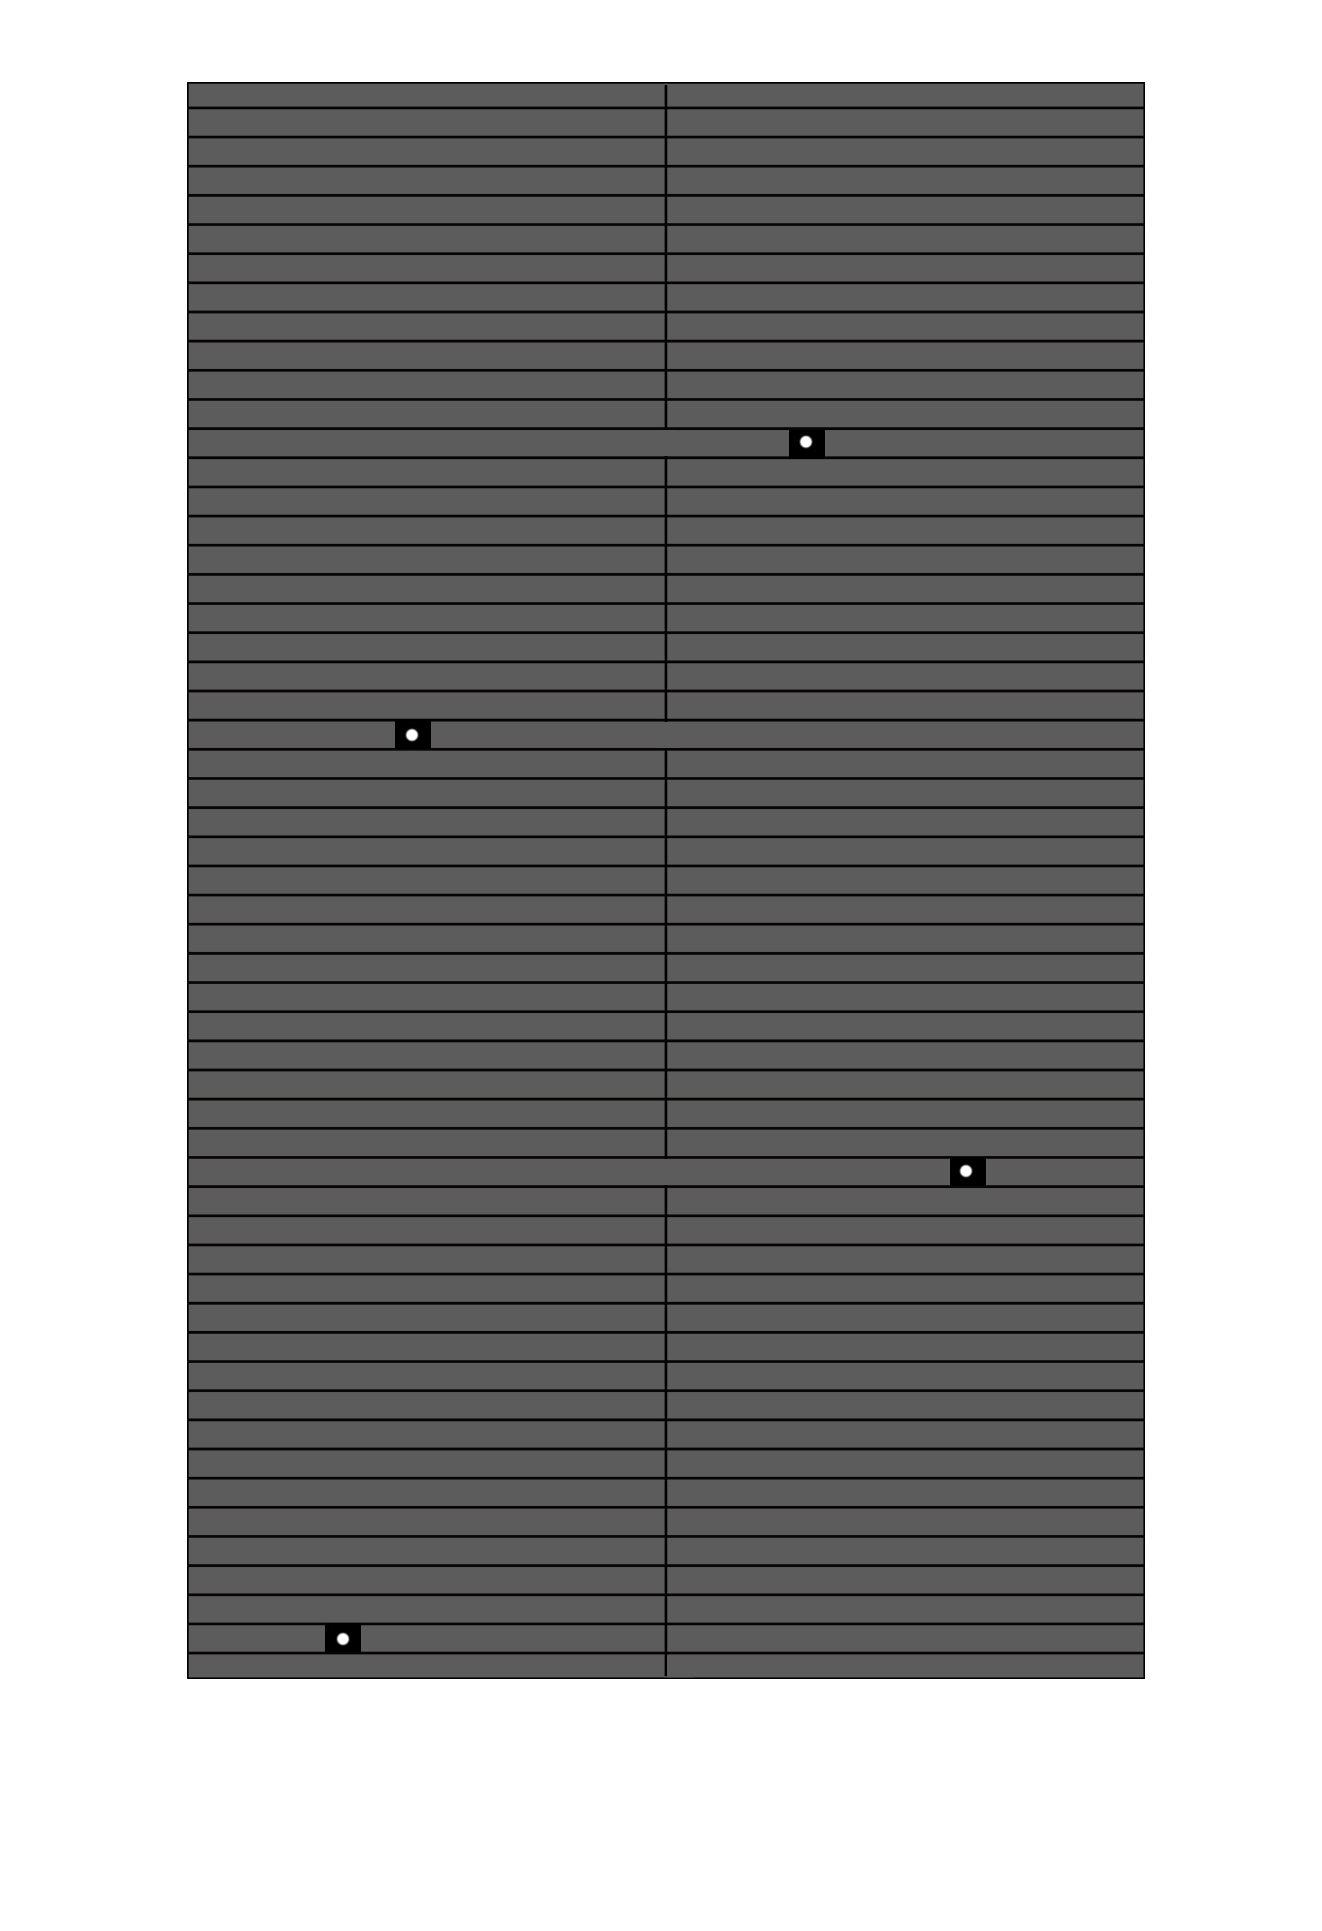
\includegraphics[height=0.5\linewidth]{CSU-puntos}
\caption{Apuntado con 4 barras ocupadas}
\label{fig:CSU2}
\end{figure}

\subsection{Beam Switching}

El \textit{beam switching} es un método para obtener mediciones de un objeto de
una forma más precisa. El método consiste (aplicado a nuestro problema) en medir
tanto la luz perteneciente al objeto celeste como la de la propia bóveda
celeste, mover a continuación ligeramente la posición del medidor (dejando los
objetos donde antes no había nada) y volver a realizar las mediciones oportunas.
La Figura \ref{fig:beams} muestra un ejemplo explicativo. De esta forma se
obtienen una serie de valores que pueden ser procesados posteriormente por el
investigador.

\begin{figure}[!htb]
\centering
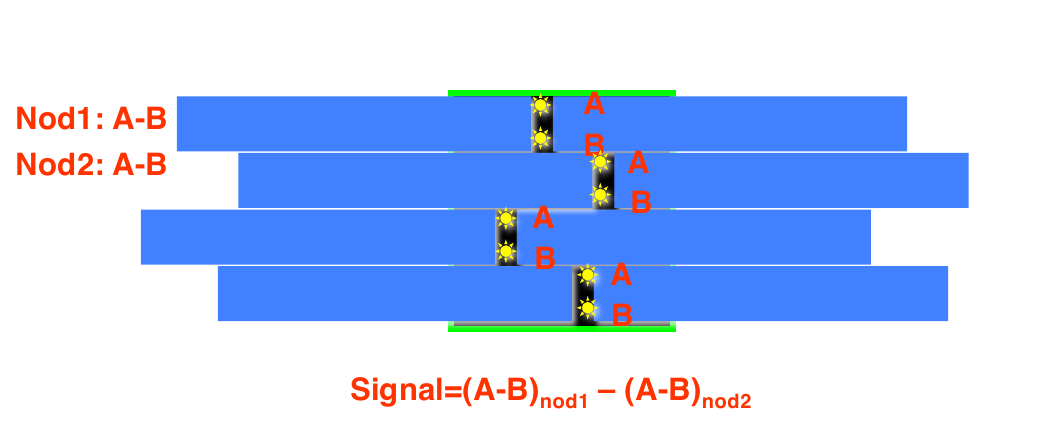
\includegraphics[width=0.7\linewidth]{beamexplication}
\caption{Muestra de funcionamiento de \texttt{beam switching}}
\label{fig:beams}
\end{figure}

